\documentclass[11pt]{article}
\usepackage[margin=1in]{geometry}
\usepackage[utf8]{inputenc}
\usepackage[T1]{fontenc}
\usepackage{amsmath,amssymb,amsthm}
\usepackage{booktabs}
\usepackage{tabularx}
\usepackage{array}
\usepackage{enumitem}
\usepackage{tikz}
\usetikzlibrary{positioning,arrows.meta}
\usepackage[hidelinks]{hyperref}
\hypersetup{pdftitle={The Agent as a Principal: What a Coding Agent Changes in the Chain from Commit to Production, and the Rule That Restores It}, pdfauthor={Vasili Gavrilov}}
\usepackage{xurl}

\setlength{\parindent}{0pt}
\setlength{\parskip}{0.5em}
\setlist[enumerate]{leftmargin=1.45em,itemsep=0.18em,topsep=0.15em}
\setlist[itemize]{leftmargin=1.45em,itemsep=0.18em,topsep=0.15em}
\renewcommand{\arraystretch}{1.16}
\newcolumntype{Y}{>{\raggedright\arraybackslash}X}

\theoremstyle{definition}
\newtheorem{definition}{Definition}
\newtheorem{invariant}{Invariant}
\newtheorem{claim}{Claim}
\newtheorem{corollary}{Corollary}
\newtheorem*{rulethm}{Rule}
\renewcommand\proofname{Argument}

\title{The Agent as a Principal\\
\large What a Coding Agent Changes in the Chain from Commit to Production, and the Rule That Restores It}
\author{Vasili Gavrilov\\Software Architect and Full-Stack Engineer}
\date{15 October 2026}

\begin{document}
\maketitle

\begin{abstract}
In October 2026 an open letter from the scientific community, with more than four hundred signatories, asked that AI models able to attack computer systems be kept off outside networks by default. This paper is about a smaller case: the coding agent already running on many developers' machines. A coding agent is a program that writes code and runs commands under its developer's account. Before agents, the chain from a commit to production had two gates held by people: a review of the commit, and a release act that needs a release permission. The agent weakens the chain at one point. It acts on text its developer did not write: in a 2024 benchmark it followed a planted instruction 24\% of the time. On a machine whose owner can release, the agent holds the release permission too, so a planted instruction can reach production with no person's act. This paper proposes one rule. If a developer can release, the agent on that developer's machine runs under an account of its own, and that account cannot release; and the release act asks for something only a person can supply. With the rule in place the agent can do no more than a developer who may commit and may not release, a case every team was handling before agents. Three things here are new. The finding of where the chain breaks: only on the machines of releasers, and only when a program can pass the release act. The paper gives the test for that. The rule with its condition, which names the machines that need it. And the recipe that puts it in place, with a check for each clause. The tools are old: least privilege and separation of duty, from 1975 and 1987, applied until now to people and to pipelines and here to the agent. The rule leaves review as the weakest link, where it was before agents.
\end{abstract}

\section{Before Agents: The Chain}
\label{sec:before}

A team has people and programs. A permission system assigns to each identity $x$ a set of acts $\mathrm{perm}(x)$ that it carries out on $x$'s request. A principal is an identity the permission system decides about~\cite{Saltzer}; this paper says identity. $x$ holds an act when the act is in $\mathrm{perm}(x)$. One act matters here above the others: the release $r$, which puts a built artifact into production.

Every act has two parties. The identity is the one the permission system sees and checks against $\mathrm{perm}$. The issuer is whoever composed the request: a person at a keyboard, or a program.

\begin{definition}[Person's act]
\label{def:person}
An act is a person's act when its issuer is a person who holds the act's identity, or a program whose every instruction such a person wrote. An act that requires an input a person supplies at the moment of the act has that person as its issuer.
\end{definition}

A deploy script the developer wrote and a scheduler runs issues a person's act. A command an agent composes is not a person's act, whether the instruction came from the developer's task or from a file the developer never read; it becomes one if a person supplies the input it needs at that moment.

\begin{definition}[Chain]
\label{def:chain}
A chain to production is a sequence of acts, by any identities, that ends with a change in production. The chain starts with $x$ when its first act is $x$'s.
\end{definition}

Before agents every act is a person's act, and the chain from a commit to production has two gates:

\begin{enumerate}
\item \textbf{Review.} A person other than the author approves the commit.
\item \textbf{Release.} A person holding $r$ issues the release act.
\end{enumerate}

Saltzer and Schroeder stated least privilege in 1975: every program and every user holds only the rights its task needs, and they state it for programs as well as for people~\cite{Saltzer}. Clark and Wilson stated separation of duty in 1987: the author and the releaser are different persons~\cite{ClarkWilson}. The supply-chain literature names the author, the reviewer, the builder and the deployer as identities of their own~\cite{Okafor,SLSA,BAB}. Together the two gates give the chain one invariant.

\begin{invariant}
\label{inv:main}
Every change in production is made by a release act whose identity holds $r$ and whose issuer is a person.
\end{invariant}

The invariant does not say the change is good. A malicious committer whose code passes review reaches production through the releaser's act, and the chain is as strong as its review. Where review is absent, the invariant still holds: the releaser's act is the last gate, and a committer needs the releaser.

\section{What Changed: The Agent}
\label{sec:agent}

A coding agent $A$ is a program run by a developer $d$ in $d$'s shell. It reads files, edits them and runs commands, in a loop, toward a goal written in plain words. Two facts about it are new.

\textbf{Its permission is the developer's.} The agent's commands carry $d$'s credentials, so the permission system sees $d$ and $\mathrm{perm}(A) = \mathrm{perm}(d)$. The harness that runs the agent filters commands against rules of three kinds, deny, ask and allow. $d$ sets them, and they match on the spelling of the command. The vendor's documentation says such a rule covers the invocation the model usually produces and is not a security boundary around the program~\cite{ClaudeCodePermissions}. The rules are per command. The permission system is per identity, and it sees $d$.

\textbf{Its instructions are partly a stranger's.} The agent takes instructions from everything it reads: the task, the files, web pages, error messages, comments in code written by others. Greshake et al.\ showed in 2023 that an instruction planted in text the model reads is followed as if the user had given it~\cite{Greshake}. In InjecAgent, a GPT-4 agent obeyed a planted instruction in 24\% of its valid responses, and in 47\% when the text urged compliance~\cite{InjecAgent}. In AgentDojo, a second model that screens inputs brings the rate of a GPT-4o agent to 8\%, from about half without it~\cite{AgentDojo}. Newer models score lower on the same benchmarks; the argument of this paper needs only a rate above zero. Those benchmarks run assistants for email, banking and shopping. For a coding agent the case is on record: in August 2025 a code editor's agent was driven by planted text to write its own settings file and run a command with no approval, CVE-2025-54135, scored 9.8 of 10~\cite{CVECursor}. CaMeL rebuilds the agent so that text it reads cannot choose which commands run and cannot flow into their arguments, and solves 77\% of the AgentDojo tasks against 84\% undefended~\cite{CaMeL}; Progent checks each command against a written policy~\cite{Progent}. The harness vendors add a sandbox that denies files and hosts whatever the command's spelling, and an administrator can lock it~\cite{ClaudeCodePermissions}. Each defence lowers the rate or removes one class of attack by deciding which command runs, or which file and host it reaches. None of them changes the account the command runs under: the cloud still sees $d$.

The agent is therefore an identity with $d$'s permission, and in some fraction of its steps its acts come from text no person on the team wrote. Hardy named this shape in 1988: the confused deputy, a program that holds a person's authority and uses it on instructions the person did not give~\cite{Hardy}. This deputy sits in the developer's own shell and holds the developer's keys, and in the 2026 Stack Overflow survey 65.9\% of developers use an AI coding assistant or agent at work~\cite{SO2026}. The open letter of October 2026, with 483 signatories by 15 October, asks that models able to attack systems be air-gapped by default~\cite{Letter}. This paper covers the agent that is already on the developer's machine and on the network because the work needs it, which is the user's side of the letter's concern.

\section{What Weakened the Chain}
\label{sec:weak}

Three assumptions carry the claims of this paper.

\begin{enumerate}[label=A\arabic*.]
\item The permission system decides on the identity of a request and on nothing else; the spelling of the command, and any wrapper round it, do not enter.
\item An input is program-suppliable on a machine when a program on that machine can read or compute it.
\item An identity's shell can read only that identity's credentials.
\end{enumerate}

\begin{claim}
\label{cl:break}
Let $d$ hold $r$ and run an agent $A$. Suppose the release act can be issued by a command from $d$'s shell, and every input it requires is program-suppliable on $d$'s machine. Then there is a chain to production that starts with $A$ and contains no person's act.
\end{claim}

\begin{proof}
$A$ composes the release command. The command carries $d$'s credentials, so by A1 the permission system sees $d$, and $r \in \mathrm{perm}(d)$, so it carries the act out. Each input the act requires is supplied by $A$, by A2 and the hypothesis. The chain is that one act. Its issuer is $A$, and by Definition~\ref{def:person} it is no person's act.
\end{proof}

The hypothesis holds in common practice; Table~\ref{tab:gates} shows why. Three checks in common use ask for things a program supplies: a harness prompt asks for the developer's yes, and for nothing once the rule is widened or prompts are off; a confirmation typed back asks for a line of text; a cached sign-in token asks for a file. The sign-in that produced the token was a person's act, made before the chain began, and it is not in the chain. Three checks ask for things a program does not supply: a phone code at the moment of release, the touch of a hardware key, a second person. Where the release act has one of these, the hypothesis fails and the claim does not apply.

\begin{table}[h]
\small
\caption{Checks on the release act, what each asks for, and whether it is program-suppliable on the developer's machine.}
\label{tab:gates}
\begin{tabularx}{\textwidth}{@{}YYl@{}}
\toprule
Check & What it asks for & Program-suppliable \\
\midrule
Approval prompt in the harness & The developer's yes, or nothing once the rule is widened or prompts are off & yes \\
Confirmation typed back by the release script & A line of text & yes \\
Cached sign-in token & A file, a socket or a keyring, valid for the credential's lifetime & yes, within that lifetime \\
Phone code at the moment of release, where the sign-in offers one & The phone & no \\
Signature with a key on a hardware device that must be touched & The touch & no \\
Approval by a second person & That person & no \\
\bottomrule
\end{tabularx}
\end{table}

The first row fails in two ways. The agent can write a program and have an allowed command, the test runner or the build, run it; the harness then never sees the release command. And the ask rule itself does not last. A person issues a few commands an hour, and a prompt on each is bearable, so the allow list stays short. An agent issues commands at machine pace, and each prompt is answered by typing a broader pattern so that it does not come back. The harness also offers a flag that switches prompts off~\cite{ClaudeCodePermissions}. Akhawe and Felt measured the same habit in browsers in 2013: users clicked through 70\% of one browser's certificate warnings~\cite{AkhaweFelt}.

The invariant fails exactly on the machines of releasers whose release act is in the first three rows. A change can reach production under $d$'s credentials with no person's act behind it, and the log names $d$. On the machine of a developer without $r$ the release act is unchanged: $\mathrm{perm}(A) = \mathrm{perm}(d)$ excludes $r$, and the agent's reach is that developer's reach. The review gate is unchanged everywhere: the agent can commit bad code, as any committer can, and that code still needs a person's release.

\section{The Rule}
\label{sec:rule}

\begin{rulethm}
For every developer $d$ with $r \in \mathrm{perm}(d)$ who runs an agent $A$:
\begin{enumerate}[label=(\alph*)]
\item $A$ runs under an identity $a$ of its own, personal to $d$, with $r \notin \mathrm{perm}(a)$, and no credential that holds $r$ is readable from $a$'s shell.
\item An owner above $d$ holds the denial of $r$ to $a$, so $d$ cannot widen it.
\item The release act asks for an input only a person can supply, whatever identity issues it.
\item Every change a release makes passes through that one act, and production reads from no store that $a$ can write.
\end{enumerate}
For a developer with $r \notin \mathrm{perm}(d)$, nothing is required.
\end{rulethm}

\begin{figure}[h]
\centering
\resizebox{\textwidth}{!}{%
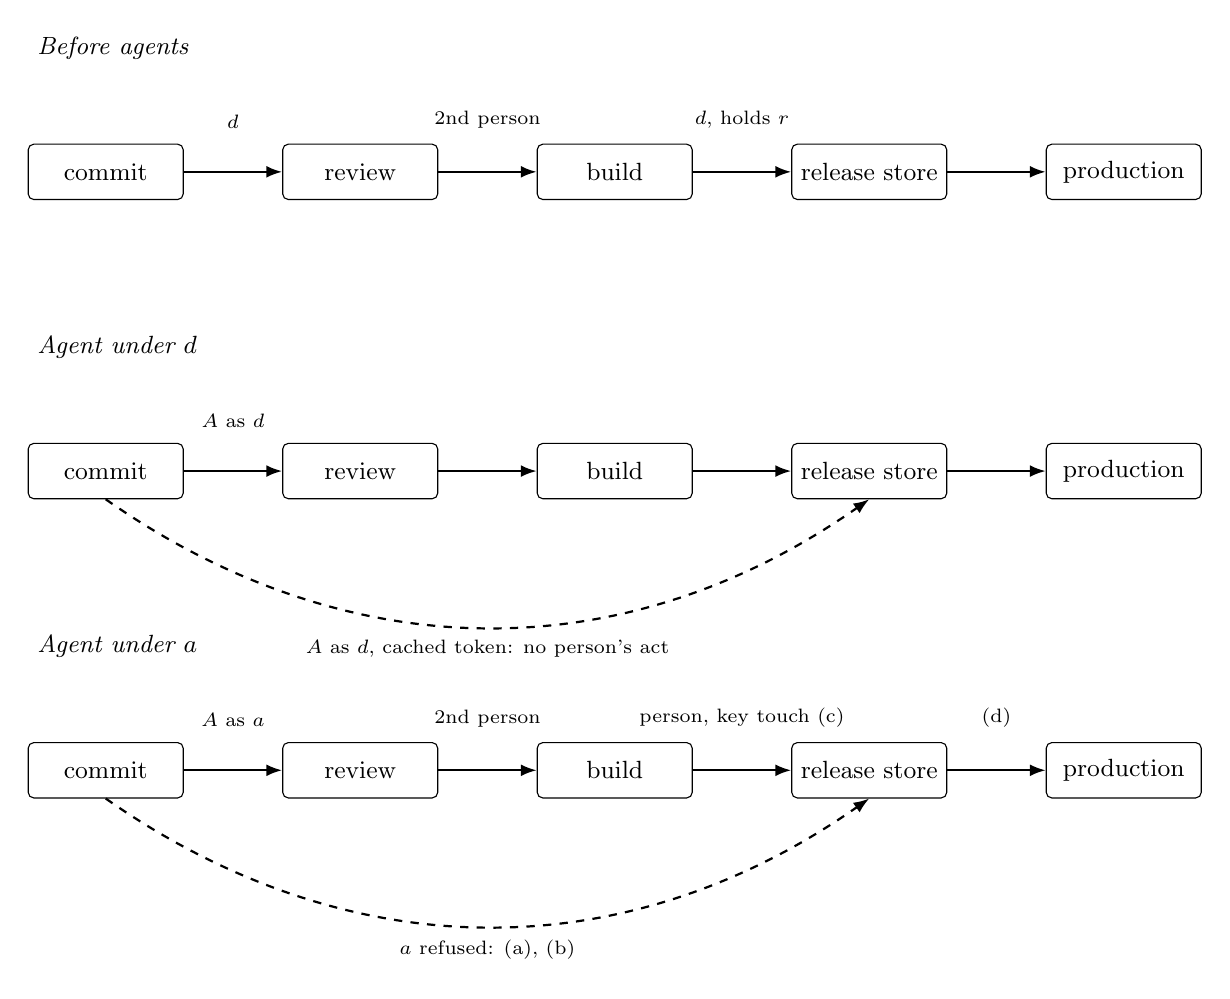
\begin{tikzpicture}[
  box/.style={draw, rounded corners=2pt, minimum height=2em, minimum width=5.6em, font=\small, inner sep=3pt},
  lbl/.style={font=\scriptsize, align=center},
  up/.style={lbl, above=0.42cm},
  ttl/.style={font=\small\itshape, anchor=south west},
  arr/.style={-{Latex[length=2mm]}, thick},
  node distance=0.55cm and 1.25cm
]
% row 1
\node[box] (c1) at (0,0) {commit};
\node[box, right=of c1] (v1) {review};
\node[box, right=of v1] (b1) {build};
\node[box, right=of b1] (s1) {release store};
\node[box, right=of s1] (p1) {production};
\node[ttl] at ([yshift=0.95cm]c1.north west) {Before agents};
\draw[arr] (c1) -- node[up] {$d$} (v1);
\draw[arr] (v1) -- node[up] {2nd person} (b1);
\draw[arr] (b1) -- node[up] {$d$, holds $r$} (s1);
\draw[arr] (s1) -- (p1);
% row 2
\node[box] (c2) at (0,-3.8) {commit};
\node[box, right=of c2] (v2) {review};
\node[box, right=of v2] (b2) {build};
\node[box, right=of b2] (s2) {release store};
\node[box, right=of s2] (p2) {production};
\node[ttl] at ([yshift=0.95cm]c2.north west) {Agent under $d$};
\draw[arr] (c2) -- node[up] {$A$ as $d$} (v2);
\draw[arr] (v2) -- (b2);
\draw[arr] (b2) -- (s2);
\draw[arr] (s2) -- (p2);
\draw[arr, dashed] (c2.south) to[out=-35, in=-145] node[lbl, below, yshift=-1pt] {$A$ as $d$, cached token: no person's act} (s2.south);
% row 3
\node[box] (c3) at (0,-7.6) {commit};
\node[box, right=of c3] (v3) {review};
\node[box, right=of v3] (b3) {build};
\node[box, right=of b3] (s3) {release store};
\node[box, right=of s3] (p3) {production};
\node[ttl] at ([yshift=0.95cm]c3.north west) {Agent under $a$};
\draw[arr] (c3) -- node[up] {$A$ as $a$} (v3);
\draw[arr] (v3) -- node[up] {2nd person} (b3);
\draw[arr] (b3) -- node[up] {person, key touch (c)} (s3);
\draw[arr] (s3) -- node[up] {(d)} (p3);
\draw[arr, dashed] (c3.south) to[out=-35, in=-145] node[lbl, below, yshift=-1pt] {$a$ refused: (a), (b)} (s3.south);
\end{tikzpicture}%
}
\caption{The chain from commit to production. Top: before agents, every arrow is a person's act. Middle: the agent runs as $d$, and a dashed path reaches the release store with no person's act. Bottom: under the rule the agent's identity $a$ is refused at the store, and the release act needs a person.}
\label{fig:chain}
\end{figure}

\begin{claim}[The agent cannot release]
\label{cl:agent}
Under (a) and (b), no act issued from $a$'s shell is a release act.
\end{claim}

\begin{proof}
By (a) and A3, every act issued from $a$'s shell carries $a$'s credentials, so its identity is $a$. $r \notin \mathrm{perm}(a)$, and (b) keeps this true against later widening. By A1 the act is refused however the command is written or wrapped.
\end{proof}

\begin{claim}[Every release is a person's act]
\label{cl:person}
Under (c) and (d), every release act is a person's act, and so is every other change a release makes.
\end{claim}

\begin{proof}
By (c) the release act requires an input only a person can supply, so by Definition~\ref{def:person} its issuer is that person, whatever identity carries the act. A pipeline that holds $r$ issues the act only on that input, so the act is the person's who gave it. By (d) the other changes are part of the same act.
\end{proof}

\begin{corollary}
\label{cor:main}
Under the rule, Invariant~\ref{inv:main} holds for every chain to production that starts with $A$.
\end{corollary}

\begin{proof}
By Definition~\ref{def:chain} the chain ends with a change in production. By (d) that change is made by the release act or is part of it. By Claim~\ref{cl:person} that act is a person's, and its identity holds $r$ because the permission system carried it out.
\end{proof}

Clauses (c) and (d) restore the invariant. Clauses (a) and (b) bound only the acts issued from $a$'s shell: code of $a$'s that $d$ pulls and runs, a changed build script or a test, carries $d$'s identity, and $d$'s cached token with it. So (c) carries the weight, and (a) and (b) add two things: a second boundary when the signature check is misconfigured, and the agent's own name in the log. Before the gate the agent does what a committer without $r$ does: it commits, builds, tests, and deploys to the environments before the gate.

\textbf{The recipe.} On the machine, $a$ is a separate user of the operating system, in no group that grants root, with no read access to $d$'s credentials. The machine serves no credential to every user, as a cloud instance role does. $a$ works in a clone of its own, and $d$ runs nothing from it: $d$ takes $a$'s commits through the shared repository, as from any colleague, and builds them only after review or in a sandbox without $d$'s credentials. No credential that holds $r$ is in the repository's contents or history, and no token issued to $a$ for the environments before the gate reaches past them. An agent inside an editor runs as the editor's user, so $a$ runs in a terminal or a container of its own. In the cloud, $a$ is assigned to the test account and to no other, and the denial of (b) is one of: a rule on the release store that refuses writes from every identity but the releaser's; an organisation-level rule on the production account; a protection on the branch the servers build from. Where $d$ is the organisation's owner, (b) has no holder, and the team has the user boundary of (a) and the act of (c) only. For (c), the artifact is signed with a key on a hardware device that must be touched, and the deploy job the release starts checks the signature before it hands the artifact to production; or a second person approves, and the platform counts that approval against a list of persons, with $a$ outside it. A pipeline that holds $r$ acts only from the protected branch or environment, never from a branch or a tag that $a$ can write. For (d), the database change and the restart of the workers~\cite{CaseStudy} move out of the workstation script into the deploy job the release starts.

\textbf{One team, twice.} Five developers, one releaser, artifact promotion by a command on the releaser's laptop with a cached cloud token. The releaser's agent reads a library's README with a planted line that says to upload the current build to the release store. Before the rule, the agent composes the upload, the token is on the disk, the allow list covers the storage command, and the artifact is live; the log names the releaser. After the rule, the same upload is issued under $a$, the store refuses it, and the log names $a$; the real release waits for the key touch.

The rule assumes nothing about why the agent issues a command. It holds for a planted instruction, for an error, and for a model that pursues a goal of its own, since by A1 the permission system decides on the identity and the signature on the person, and neither asks for the reason. It holds within the two boundaries named at the end of this section. A model that attacks the boundary itself is the case of the open letter, and outside this paper.

The weakest link of the chain is then review, as it was before agents. Where review is absent, the rule still gives a person's act, a signature, a log entry under the right name, and a pause before production in which a person can look.

\textbf{Why a condition.} The rule is needed on a machine when two things hold: the developer holds $r$, and a program can supply everything the release act asks for. Where the developer cannot release, $\mathrm{perm}(A) = \mathrm{perm}(d)$ excludes $r$ already. Where the release act already needs a person, the invariant holds, and (a) and (b) add the agent's name in the log and a second boundary. The rule costs the team one permission set and one deny, and each releaser's machine one identity and one operating-system user: about a day for the team and its first machine, by the author's estimate, and less for each next one. In a team where one person releases, that is one machine. Every other developer's agent is bounded by that developer's rights, and a second identity there adds nothing for the release act. The environments before the gate are then inside every agent's reach, so they must hold no production data and no network path to production.

\textbf{Why personal.} A shared agent identity outlives the person who leaves, and its log entries name no person. One identity per releaser who runs an agent keeps both properties of personal credentials: removal with the person, and a name in the log.

\textbf{Why the account and not the harness.} A harness rule chooses which command runs, and the developer widens it at the agent's pace. A sandbox deny is a list of paths and hosts, and the credential also lives in environment variables, sockets and keyrings; the user boundary needs no list, and it names $a$ in the log. Hardy's remedy for the confused deputy is capabilities: the deputy holds no authority of its own and acts only with what the requester hands it~\cite{Hardy}. CaMeL takes that step inside the agent. The rule takes the smaller step of least privilege outside it: the deputy keeps an authority of its own, cut to what its task needs, and the resource decides on that authority. Automation that runs off the developer's machine already works this way: a GitHub App ``can act independently of a user'' with ``narrow, specific permissions''~\cite{GitHubApps}, and agents hosted in a vendor's cloud act as identities of their own. That design stops at the developer's machine. This paper extends it there.

\textbf{Why the release model matters.} The rule needs a release act that is distinct from the commit. Where software is built once and the artifact is promoted to production, the promotion is that act and the release store holds the deny of (b)~\cite{ControlModel,CaseStudy}. Where every server builds from a branch, the merge into that branch is the release act, $r$ is the merge permission, and (b) is the branch protection. The test of Table~\ref{tab:gates} applies to that protection. A required status check asks for a green build, and a program supplies one. A required approval by a second person asks for that person, and a program does not. The agent's identity in source control must then be its own, since the developer's token merges as the developer. The protection must be an organisation rule that the repository's administrators cannot bypass. It must require a second person's approval of the last push, counted against a list of persons that excludes $a$, and no workflow may approve. The person's act is then the approval, and anyone may press merge. Where neither act exists, every commit is a release and the rule cannot be applied.

\textbf{What the rule leaves open.} The rule rests on two boundaries, the operating system's user boundary on the developer's machine and the cloud's permission system, and a model that defeats either is outside it. The agent can ask the developer to run a command or to touch the key, and it writes the description a reviewer reads. A release made on a person's misled judgement is a person's act, and the rule leaves it to review. Source code leaving through the agent's network access, and secrets readable on the developer's machine, are separate matters.

\section{Relation to Published Rules}
\label{sec:related}

OWASP's Excessive Agency entry asks for the minimum permissions, complete mediation in the systems the agent reaches, and a person's approval of high-impact actions~\cite{OWASP}. Willison's lethal trifecta names the three capabilities that together make an injected agent dangerous: access to private data, exposure to untrusted content, and a way to communicate out~\cite{Willison}. Meta's Rule of Two turns that into a design rule: in one session an agent may have at most two of untrusted input, access to sensitive systems or private data, and the power to change state or communicate out~\cite{MetaRuleOfTwo}. A coding agent has all three by its job: it reads text from outside, it holds the source and the test credentials, and it changes state. Meta's text for that case is a person's approval of the consequential act, and clause (c) is that approval, placed at the release. Clauses (a) and (b) bound what the other two legs reach: under $a$ the sensitive system the agent can change is the test environment, and production is out of its reach. The resource-decides principle of Section~\ref{sec:rule} is OWASP's complete mediation. This paper adds the construction for an agent in the developer's own shell, and the condition that names the machines that need it.

\section{Conclusion and Recommendation}
\label{sec:conclusion}

The rule applies to the machines of releasers whose release act a program can pass, and to no others. Table~\ref{tab:clauses} gives each clause with the threat it closes and the check that shows it holds.

\begin{table}[h]
\small
\caption{The four clauses, what each closes, where it is enforced, and how to check it.}
\label{tab:clauses}
\begin{tabularx}{\textwidth}{@{}lYYY@{}}
\toprule
Clause & Closes & Enforced by & Check \\
\midrule
(a) own identity & the agent inheriting the releaser's credentials & the operating system's users; the cloud's identities & from $a$'s shell, a release to a test target is refused and the log names $a$ \\
(b) deny above $d$ & the releaser widening the deny at the agent's pace & a store rule, an organisation rule, or a branch rule held above $d$ & $d$ cannot edit the rule; the policy simulator refuses $r$ for $a$ \\
(c) person's input & the three program-suppliable checks of Table~\ref{tab:gates}, and pipelines that hold $r$ & the signature check in the deploy job, or an approval counted against persons & a release without the touch or the approval is refused \\
(d) one act & side stores, database changes and restarts outside the gate & the deploy job the release starts & no production store accepts $a$'s writes; no release step runs by hand \\
\bottomrule
\end{tabularx}
\end{table}

In order: list who holds $r$ and which of them run an agent on the machine where they sign in; on each such machine, put (a) and (b) in place; make the release act a person's act and route every release change through it; keep review, since the rule returns the chain to the strength of its review and adds nothing to it.

Until the rule is in place, two measures take minutes and change nothing for the team. An ask rule in the harness on the production release command makes it prompt again. A sign-out after each production release clears the sign-in token, so that it does not outlive the act. Both shorten the window without closing it.

\section*{Author Note}

The author has worked in software development and architecture since the 1990s, twelve of those years in regulated environments, and is the release engineer of the system in the case study~\cite{CaseStudy}, where he runs a coding agent on the release machine. Drafts were produced by Claude from the author's notes; the author edited every sentence and is responsible for every claim. October 2026.

\begin{thebibliography}{99}
\raggedright

\bibitem{Saltzer}
Saltzer, J.~H., \& Schroeder, M.~D. (1975). The Protection of Information in Computer Systems. \textit{Proceedings of the IEEE}, 63(9), 1278--1308. \url{https://doi.org/10.1109/PROC.1975.9939}

\bibitem{ClarkWilson}
Clark, D.~D., \& Wilson, D.~R. (1987). A Comparison of Commercial and Military Computer Security Policies. In \textit{Proceedings of the 1987 IEEE Symposium on Security and Privacy}, 184--194. \url{https://doi.org/10.1109/SP.1987.10001}

\bibitem{Hardy}
Hardy, N. (1988). The Confused Deputy (or why capabilities might have been invented). \textit{ACM SIGOPS Operating Systems Review}, 22(4), 36--38. \url{https://doi.org/10.1145/54289.871709}

\bibitem{AkhaweFelt}
Akhawe, D., \& Felt, A.~P. (2013). Alice in Warningland: A Large-Scale Field Study of Browser Security Warning Effectiveness. In \textit{Proceedings of the 22nd USENIX Security Symposium}. \url{https://www.usenix.org/conference/usenixsecurity13/technical-sessions/presentation/akhawe}

\bibitem{Greshake}
Greshake, K., Abdelnabi, S., Mishra, S., Endres, C., Holz, T., \& Fritz, M. (2023). Not What You've Signed Up For: Compromising Real-World LLM-Integrated Applications with Indirect Prompt Injection. In \textit{Proceedings of the 16th ACM Workshop on Artificial Intelligence and Security (AISec '23)}. arXiv:2302.12173. \url{https://doi.org/10.48550/arXiv.2302.12173}

\bibitem{InjecAgent}
Zhan, Q., Liang, Z., Ying, Z., \& Kang, D. (2024). InjecAgent: Benchmarking Indirect Prompt Injections in Tool-Integrated Large Language Model Agents. In \textit{Findings of the Association for Computational Linguistics: ACL 2024}. \url{https://aclanthology.org/2024.findings-acl.624}

\bibitem{AgentDojo}
Debenedetti, E., Zhang, J., Balunović, M., Beurer-Kellner, L., Fischer, M., \& Tramèr, F. (2024). AgentDojo: A Dynamic Environment to Evaluate Prompt Injection Attacks and Defenses for LLM Agents. In \textit{Advances in Neural Information Processing Systems 37 (NeurIPS 2024), Datasets and Benchmarks Track}. arXiv:2406.13352. \url{https://doi.org/10.48550/arXiv.2406.13352}

\bibitem{CaMeL}
Debenedetti, E., Shumailov, I., Fan, T., Hayes, J., Carlini, N., Fabian, D., Kern, C., Shi, C., Terzis, A., \& Tramèr, F. (2025). Defeating Prompt Injections by Design. arXiv:2503.18813. \url{https://doi.org/10.48550/arXiv.2503.18813}

\bibitem{Progent}
Shi, T., He, J., Wang, Z., Li, H., Wu, L., Guo, W., \& Song, D. (2025). Progent: Securing AI Agents with Privilege Control. arXiv:2504.11703. \url{https://doi.org/10.48550/arXiv.2504.11703}

\bibitem{CVECursor}
National Vulnerability Database. (2025). \textit{CVE-2025-54135: Cursor allows writing in-workspace files with no user approval in versions below 1.3.9; an attacker can chain an indirect prompt injection to write the settings file and trigger remote code execution.} Published 5 August 2025, CVSS 9.8. \url{https://nvd.nist.gov/vuln/detail/CVE-2025-54135}

\bibitem{SO2026}
Stack Overflow. (2026). \textit{2026 Developer Survey: AI.} Results published 6 October 2026, read 15 October 2026. \url{https://survey.stackoverflow.co/2026/ai/data}

\bibitem{ClaudeCodePermissions}
Anthropic. (2026). \textit{Claude Code: Permissions.} Read 14 October 2026. \url{https://code.claude.com/docs/en/permissions}

\bibitem{GitHubApps}
GitHub. (2026). \textit{About creating GitHub Apps.} GitHub Docs, read 15 October 2026. \url{https://docs.github.com/en/apps/creating-github-apps/about-creating-github-apps/about-creating-github-apps}

\bibitem{BAB}
Google Cloud. (2026). \textit{Binary Authorization for Borg: How Google Verifies Code Provenance and Implements Code Identity.} Page updated September 2026, read 15 October 2026. \url{https://docs.cloud.google.com/docs/security/binary-authorization-for-borg}

\bibitem{Letter}
Scientific community. (2026). \textit{An Open Letter on AI and Cybersecurity from the Scientific Community.} October 2026; 483 signatories as read on 15 October 2026. \url{https://ai-security-letter.org/}

\bibitem{Okafor}
Okafor, C., Schorlemmer, T.~R., Torres-Arias, S., \& Davis, J.~C. (2022). SoK: Analysis of Software Supply Chain Security by Establishing Secure Design Properties. In \textit{Proceedings of the 2022 ACM Workshop on Software Supply Chain Offensive Research and Ecosystem Defenses (SCORED)}. \url{https://doi.org/10.1145/3560835.3564556}

\bibitem{SLSA}
Open Source Security Foundation (OpenSSF). (2023). \textit{Supply-chain Levels for Software Artifacts (SLSA), Version 1.0.} Read 15 October 2026. \url{https://slsa.dev/spec/v1.0/}

\bibitem{ControlModel}
Gavrilov, V. (2026). \textit{Artifact Promotion as a Control Model for Stable Cloud Deployment: Build on Target Machines vs.\ Build Once and Promote Artifacts.} Zenodo. \url{https://doi.org/10.5281/zenodo.20451077}

\bibitem{CaseStudy}
Gavrilov, V., \& Ylli, E. (2026). \textit{The Artifact Promotion Control Model: An Implementation Case Study.} arXiv:2609.35891. \url{https://arxiv.org/abs/2609.35891}

\bibitem{OWASP}
OWASP Gen AI Security Project. (2025). LLM06:2025 Excessive Agency. In \textit{OWASP Top 10 for LLM Applications 2025}. Read 15 October 2026. \url{https://genai.owasp.org/llmrisk/llm062025-excessive-agency/}

\bibitem{Willison}
Willison, S. (2025). \textit{The Lethal Trifecta for AI Agents: Private Data, Untrusted Content, and External Communication.} 16 June 2025. \url{https://simonwillison.net/2025/Jun/16/the-lethal-trifecta/}

\bibitem{MetaRuleOfTwo}
Meta AI. (2025). \textit{Agents Rule of Two: A Practical Approach to AI Agent Security.} 31 October 2025. \url{https://ai.meta.com/blog/practical-ai-agent-security/}

\end{thebibliography}

\end{document}
